\subsection{VLA Offline Evaluation}\label{sec:vla-eval}

One \emph{partial} blue-target demonstration yielded 340 frames at 10~Hz. SmolVLA was fine-tuned for 100 BF16 steps with batch size~1 and a frozen vision encoder; the resulting checkpoint was successfully reloaded. On nine sampled frames from the \emph{same training episode} (indices 0, 20, 50, 100, 150, 200, 250, 300, and 339), linear and angular velocity MAEs relative to teacher commands were 0.0141~m/s and 0.0281~rad/s, respectively (Fig.~\ref{fig:smartcam_vla_velocity}). Initial turning and stopping remain error modes.

These are \emph{in-sample offline action imitation results}, not evidence of successful closed-loop VLA navigation, generalization, or physical robot deployment. Goal completion was not verified, and the trained VLA has not controlled the simulated or physical robot.

\begin{figure}[!t]
    \centering
    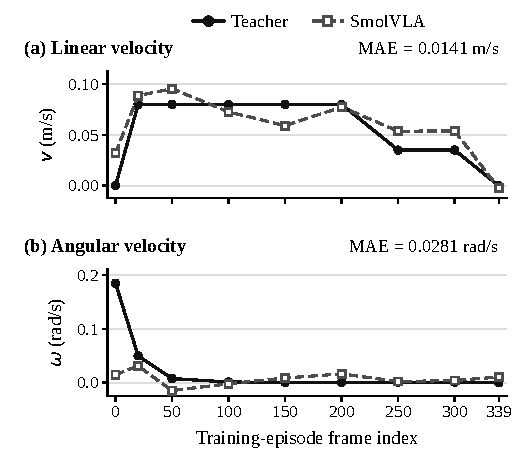
\includegraphics[width=\columnwidth]{images/vla_offline_velocity_comparison_ieee.pdf}
    \caption{Rule-based teacher commands and SmolVLA offline predictions on nine frames from the same training episode: (a) linear velocity and (b) angular velocity. Dashed curves connect sampled predictions; this is an in-sample action comparison, not a closed-loop navigation result.}
    \label{fig:smartcam_vla_velocity}
\end{figure}

